\section{Estudo de caso}
\subsection{Processo industrial de manufatura}
Descrição do Processo Fig. \ref{fig:processo}
\subsection{Solução proposta}
\begin{figure}[H]%
    \centering
    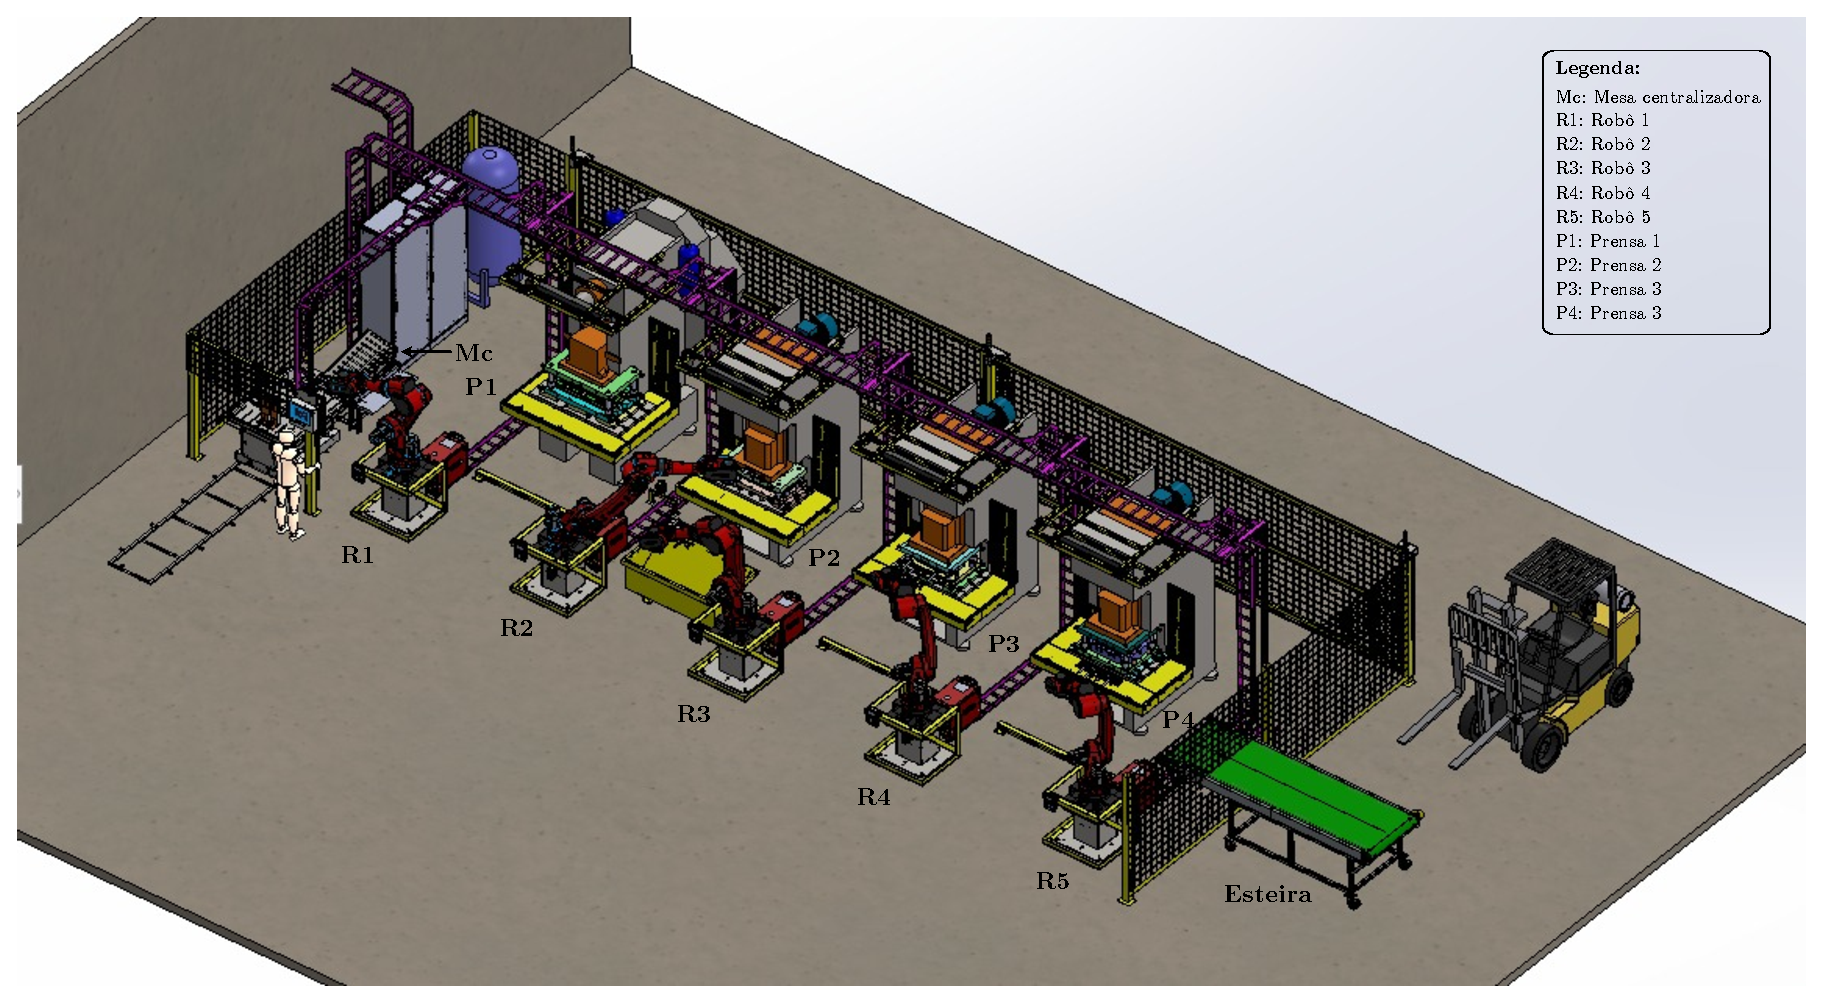
\includegraphics[width=0.8\textwidth]{imagens/processo.eps}
    \caption{Planta industrial}\label{fig:processo}
\end{figure}
\subsection{Plantas}
Robo 1 Fig \ref{fig:robo1}
\begin{figure}[H]%
    \centering
    \includegraphics[width=0.9\textwidth]{imagens/robo_1.eps}
    \caption{Planta Robo 1}\label{fig:robo1}
\end{figure}

\section{Especificações}
Especificação 1 Fig. \ref{fig:especificacao1} direciona a mesa centralizadora e robo 1 com base no sensor de chapas duplas.
\begin{figure}[H]%
    \centering
    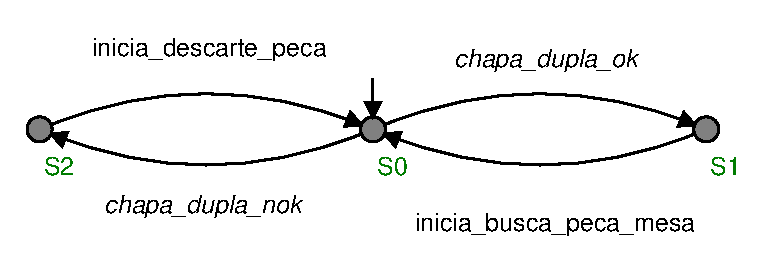
\includegraphics[width=0.9\textwidth]{imagens/E1_robo_1_chapa_dupla.eps}
    \caption{Planta Robo 5}\label{fig:especificacao1}
\end{figure}